% FLAMINGO m9 resolution and the IA spectra: whether the 2.8 Gpc box can replace or extend L1_m8.
% Build with assets/build_note.sh of the summary-notes skill.
\documentclass[11pt]{article}

\usepackage[margin=1in]{geometry}
\usepackage{amsmath}
\usepackage{amssymb}
\usepackage{graphicx}
\usepackage{booktabs}
\usepackage{xcolor}
\usepackage[font=small,labelfont=bf,labelsep=period]{caption}
\usepackage[hidelinks]{hyperref}

% Symbols, one macro per object.
\newcommand{\hMpc}{\,h\,{\rm Mpc}^{-1}}
\newcommand{\Mpch}{\,h^{-1}{\rm Mpc}}
\newcommand{\Msun}{\,M_\odot}
\newcommand{\Mstar}{M_\ast}
\newcommand{\Nstar}{N_\ast}
\newcommand{\anla}{a_{\rm NLA}}
\newcommand{\PdE}{P_{\delta E}}
\newcommand{\PhE}{P_{hE}}
\newcommand{\erms}{e_{\rm rms}}
\newcommand{\run}[1]{\texttt{#1}}

% =====================================================================
% Numbers
% =====================================================================
% Every number the text quotes is defined here, with the file (and key)
% it comes from. Paths are relative to flamingo/resolution_tests/.
% Part 1: results, refreshed when the tests are rerun; set
% \numbersfinalfalse to print them in red while they are stale.
% Part 2: inputs and simulation facts, which a rerun does not change.
%
% Statements of the text that rest on Part 1 (re-check after a refresh):
%   - m9 shapes exist (100 stars) only above log M* ~ 10.9 (section "The
%     100-star floor").
%   - At high mass the same-volume m9/m8 a_NLA ratio equals the e_rms
%     ratio (section "High mass").
%   - At log M* ~ 10, m9 keeps less than half of the signal and its shapes
%     are unrelated to the m8 shapes of the same galaxies (section "Low mass").
%   - Counting noise alone explains only a 10% loss (same section).
%   - The 2.8 Gpc box reaches S/N >= 3 per bin at k ~ 0.011 with m8-quality
%     galaxies and ~0.02 with the m9 galaxies, against 0.036 for L1_m8
%     (section "Low k").
\newif\ifnumbersfinal
\numbersfinaltrue
\newcommand{\refresh}[1]{\ifnumbersfinal#1\else\textcolor{red}{#1}\fi}
% ---- Part 1: results ----
% particle masses and the 100-star mass (particle_count.json: mstar_particle, logM_at_100)
\newcommand{\mStarMnine}{\refresh{\ensuremath{7.6\times10^{8}}}}
\newcommand{\mStarMeight}{\refresh{\ensuremath{8.9\times10^{7}}}}
\newcommand{\logMhundredMnine}{\refresh{10.88}}
\newcommand{\logMhundredMeight}{\refresh{9.95}}
% median N* at log M* = 10.0 to 10.25 (particle_count.json: bins[logM=10.125].Nstar_med)
\newcommand{\NstarTenMnine}{\refresh{18}}
\newcommand{\NstarTenMeight}{\refresh{144}}
% high-mass test (restest_L1m9/results.json: anla, anla_err, erms, ngal)
\newcommand{\anlaHMeight}{\refresh{\ensuremath{6.80 \pm 0.11}}}
\newcommand{\anlaHMnine}{\refresh{\ensuremath{5.97 \pm 0.10}}}
\newcommand{\anlaHLtwo}{\refresh{\ensuremath{5.69 \pm 0.02}}}
\newcommand{\ermsHMeight}{\refresh{0.153}}
\newcommand{\ermsHMnine}{\refresh{0.136}}
\newcommand{\ratioHM}{\refresh{0.877}}
\newcommand{\ermsratioHM}{\refresh{0.886}}
\newcommand{\NgalHMeight}{\refresh{99\,877}}
\newcommand{\NgalHMnine}{\refresh{85\,473}}
% high-mass matched galaxies (restest_L1m9/match.json: matched, proj.z.corr, proj.z.pa_med)
\newcommand{\matchHM}{\refresh{79\,504}}
\newcommand{\matchHMfrac}{\refresh{80\%}}
\newcommand{\corrHM}{\refresh{0.59}}
\newcommand{\paHM}{\refresh{\ensuremath{19^\circ}}}
% low-mass test (lowmass_L1m9/results.json: summary.*, ratios.*.anla_ratio, matched)
\newcommand{\anlaLMeight}{\refresh{\ensuremath{1.864 \pm 0.034}}}
\newcommand{\anlaLMnine}{\refresh{\ensuremath{0.844 \pm 0.043}}}
\newcommand{\anlaLMeightMatch}{\refresh{\ensuremath{1.679 \pm 0.046}}}
\newcommand{\anlaLMnineMatch}{\refresh{\ensuremath{0.682 \pm 0.072}}}
\newcommand{\ratioLM}{\refresh{0.45}}
\newcommand{\ratioLMmatch}{\refresh{0.41}}
\newcommand{\NgalLMeight}{\refresh{2.03}}
\newcommand{\NgalLMnine}{\refresh{3.03}}
\newcommand{\NgalLMmatch}{\refresh{1.22}}
\newcommand{\matchLMfrac}{\refresh{60\%}}
\newcommand{\biasLMeight}{\refresh{1.15}}
\newcommand{\biasLMnine}{\refresh{0.97}}
\newcommand{\ermsLMeight}{\refresh{0.250}}
\newcommand{\ermsLMnine}{\refresh{0.372}}
\newcommand{\NstarLMeight}{\refresh{175}}
\newcommand{\NstarLMnine}{\refresh{22}}
\newcommand{\corrLM}{\refresh{0.035}}
\newcommand{\corrLMlow}{\refresh{0.025}}
\newcommand{\corrLMhigh}{\refresh{0.070}}
\newcommand{\paLM}{\refresh{\ensuremath{43.5^\circ}}}
% counting-noise Monte Carlo at N = 20 (discreteness_mc.json: rows[N=20])
\newcommand{\mcResponseTwenty}{\refresh{0.91}}
\newcommand{\mcNoiseTwenty}{\refresh{0.33}}
% low-k forecast (lowk_forecast.json): first bin with S/N >= 3
\newcommand{\kSNLone}{\refresh{0.036}}
\newcommand{\kSNideal}{\refresh{0.011}}
\newcommand{\kSNmnine}{\refresh{0.020}}
% L1_m8 z = 0 a_NLA of the production run (FLAMINGO_IA_update_2026-10-27, table)
\newcommand{\anlaProd}{\ensuremath{1.856 \pm 0.034}}
% ---- Part 2: inputs and simulation facts ----
\newcommand{\LoneBox}{681.0}
\newcommand{\LtwoBox}{1906.8}
\newcommand{\kfLone}{0.0092}
\newcommand{\kfLtwo}{0.0033}
\newcommand{\NstarsLeight}{\ensuremath{5.04\times10^{9}}}
\newcommand{\NstarsLnine}{\ensuremath{0.54\times10^{9}}}
\newcommand{\NstarsLtwo}{\ensuremath{1.19\times10^{10}}}

\begin{document}

\begin{center}
  {\LARGE FLAMINGO m9 resolution and the IA spectra\par}
  \vspace{0.6em}
  {\large Can the 2.8 Gpc box (\run{L2p8\_m9}) replace or extend \run{L1\_m8}?\par}
  \vspace{0.6em}
  {\large November 2026\par}
  \ifnumbersfinal\else
    \vspace{0.6em}
    {\color{red}Numbers in red are being refreshed.\par}
  \fi
\end{center}
\vspace{1em}

\section{Summary}
\label{sec:summary}

\paragraph{The question.}
The IA spectra of the paper come from \run{L1\_m8} (1~Gpc box, star particles of
$\sim\!10^{8}\Msun$) for galaxies with $\log_{10}\Mstar/\Msun \gtrsim 10$. Can the
2.8~Gpc box \run{L2p8\_m9}, with 8 times heavier particles, measure the same
spectra and extend them to lower $k$?

\paragraph{The answer.}
Not for this sample. At $\log\Mstar \simeq 10$ an m9 galaxy has about
\NstarTenMnine{} star particles, and in the same volume its alignment signal is
\ratioLMmatch{} to \ratioLM{} of the m8 one (Figure~\ref{fig:lowmass_ratio});
the shapes of the same galaxies at the two resolutions are unrelated (shape
correlation \corrLM). At high mass ($\Mstar > 4\times10^{11}\Msun$, more than 500
particles) the m9 deficit is only $1-\ratioHM = 12\%$.

\paragraph{Why.}
The earlier claim that m9 has too few particles holds: with star particles of
\mStarMnine$\Msun$, SOAP's 100-particle shape mask sits at
$\log\Mstar = \logMhundredMnine$ (Section~\ref{sec:count}, The 100-star floor).
Shapes can be measured from fewer particles, and counting noise alone costs only
10\% of the signal at 20 particles. The loss measured is larger because the m9
galaxies themselves differ: \run{L1\_m9} shares its initial phases with
\run{L1\_m8}, so the two runs can be compared galaxy by galaxy, and at low mass
the m9 orientations are random with respect to the m8 ones
(Section~\ref{sec:lowmass}, Low mass). A correction of a factor 2.2 to 2.5 that
changes with $k$ and with the population is not a measurement.

\paragraph{Limits.}
The tests are at $z = 0$ only. m8 itself is not shown to be converged (there is
no higher-resolution FLAMINGO run). The low-$k$ reach is a Gaussian forecast
(Section~\ref{sec:lowk}, What the 2.8 Gpc box adds at low k).

\section{Setup and definitions}
\label{sec:setup}

\paragraph{Runs.}
FLAMINGO hydrodynamical runs; their halo catalogues (SOAP, built on HBT) and
particle snapshots are streamed from the COSMA data server:
\begin{center}
  \begin{tabular}{lccc}
    \toprule
    run & box [$\Mpch$] & star particle [$\Msun$] & stars at $z=0$ \\
    \midrule
    \run{L1\_m8}   & \LoneBox & \mStarMeight & \NstarsLeight \\
    \run{L1\_m9}   & \LoneBox & \mStarMnine  & \NstarsLnine \\
    \run{L2p8\_m9} & \LtwoBox & \mStarMnine  & \NstarsLtwo \\
    \bottomrule
  \end{tabular}
\end{center}
Star particle masses are the median of $\Mstar/\Nstar$. The m8 version of the
2.8~Gpc box (FLAMINGO-10K) is dark matter only and has a SOAP catalogue at $z=0$
only, so it carries no galaxy shapes. \run{L1\_m8} and \run{L1\_m9} start from
the same initial phases: their five most massive clusters lie at the same
positions to $0.1\Mpch$. Their ratio is therefore a resolution test with most of
the cosmic variance removed.

\paragraph{Shapes and samples.}
Ellipticities projected along $z$, $e_1 = (I_{xx}-I_{yy})/(I_{xx}+I_{yy})$ and
$e_2 = 2I_{xy}/(I_{xx}+I_{yy})$. Two tests:
\begin{itemize}
  \item \textbf{high mass}: $\Mstar > 4.05\times10^{11}\Msun$, SOAP tensor
    \texttt{StellarInertiaTensorNoniterative} (bound stars within one stellar
    half-mass radius), which SOAP stores only for $\Nstar \ge 100$;
  \item \textbf{low mass}: $10.0 < \log\Mstar < 10.41$ (the $z=0$ bin of the
    paper's sample), unreduced inertia tensor of all bound star particles
    (the TNG definition used for the paper), computed from the particles by
    \texttt{particle\_shapes.py} with at least 10 stars at m9 and 100 at m8.
\end{itemize}
Same galaxies: an m8 galaxy is paired with the nearest m9 galaxy within
$0.2\Mpch$ and 0.3~dex in $\Mstar$; pairs sharing an m9 galaxy are dropped.

\paragraph{The statistic.}
$\PhE$ is measured on a $512^3$ grid (folded 4 times above $k = 0.8\hMpc$),
$\PdE = \PhE/b(k)$ with $b(k)^2 = (P_{hh} - V/N)/P_{\rm NL}$, in shear units. The
NLA amplitude comes from a fit $\PdE = -\anla\, C_1\rho_{\rm cr}\,\Omega_m\,
P_{\rm NL}(k)/D(z)$ at $k = 0.05$ to $0.3\hMpc$, $C_1\rho_{\rm cr} = 0.0134$,
as in the production run. Errors are the mode scatter of the spectra.

\section{The 100-star floor puts m9 shapes above $\log \Mstar = 10.9$}
\label{sec:count}

At m9 the SOAP shape mask of 100 star particles is reached at
$\log\Mstar = \logMhundredMnine$, against \logMhundredMeight{} at m8
(Figure~\ref{fig:particle_count}). In the lowest bin of the paper's sample,
$\log\Mstar = 10.0$ to $10.25$, the median galaxy has \NstarTenMnine{} star
particles at m9 and \NstarTenMeight{} at m8. \run{L1\_m9} and \run{L2p8\_m9}
give the same relation, as they share resolution and subgrid model.

\begin{figure}[tbp]
  \centering
  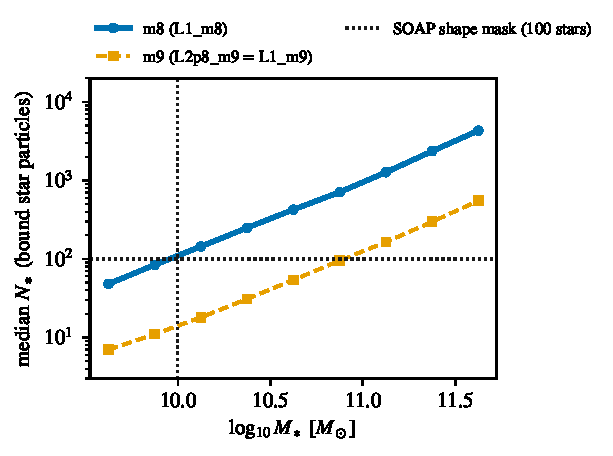
\includegraphics[width=3.5in]{plots/particle_count/particle_count.pdf}
  \caption{Median number of bound star particles per subhalo against stellar
    mass at $z=0$, in bins of 0.25~dex, for m8 (solid, circles) and m9 (dashed,
    squares; \run{L1\_m9} is identical and not drawn). Dotted: the
    100-particle SOAP shape mask and the lower edge of the paper's sample,
    $\log\Mstar = 10$.}
  \label{fig:particle_count}
\end{figure}

\section{High mass: m9 alignments are 12\% low, as much as m9 shapes are rounder}
\label{sec:highmass}

Above $\Mstar = 4\times10^{11}\Msun$, where both resolutions have SOAP shapes,
\run{L1\_m9} gives $\anla = \anlaHMnine$ against \anlaHMeight{} for
\run{L1\_m8} in the same volume, a ratio of \ratioHM{}
(Figure~\ref{fig:m9_m8_ratio}). The ratio of $\erms$ is \ermsratioHM{}
(\ermsHMnine{} against \ermsHMeight): the m9 galaxies are rounder within one
half-mass radius, and the alignment amplitude is lower by the same factor. The
ratio of the spectra is flat from $k = 0.1$ to $1\hMpc$ within the errors.

\run{L2p8\_m9} gives $\anla = \anlaHLtwo$. An earlier comparison of
\run{L2p8\_m9} with \run{L1\_m8} found a 16\% deficit; about 5 of those 16
points are cosmic variance between the two boxes, which the same-phase pair
removes.

Galaxy by galaxy, \matchHM{} of the \NgalHMeight{} m8 galaxies
(\matchHMfrac) have an m9 counterpart. Their shapes correlate at \corrHM{},
with a median position-angle offset of \paHM: individual shapes are not
converged, but the part aligned with the tidal field is, up to the rounding.

\begin{figure}[tbp]
  \centering
  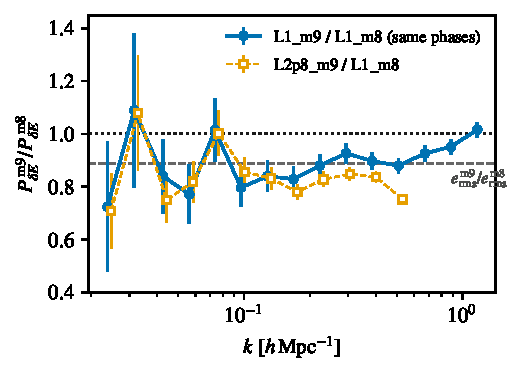
\includegraphics[width=3.5in]{plots/m9_m8_ratio/m9_m8_ratio.pdf}
  \caption{Ratio of $\PdE$ at m9 to m8 for $\Mstar > 4.05\times10^{11}\Msun$,
    $z=0$, SOAP one-half-mass-radius tensor. Filled circles: \run{L1\_m9}
    over \run{L1\_m8} (same initial phases). Open squares: \run{L2p8\_m9} over
    \run{L1\_m8}, interpolated to the L1 bins, shown below 0.7 times the
    Nyquist frequency of its grid. Dotted: 1; dashed: the ratio of $\erms$.
    Error bars add the two mode-scatter errors in quadrature, an overestimate
    for the same-phase pair. Below $k = 0.08\hMpc$ both ratios share the
    scatter of the common denominator.}
  \label{fig:m9_m8_ratio}
\end{figure}

\section{Low mass: m9 keeps less than half of the alignment signal}
\label{sec:lowmass}

In the paper's $z=0$ bin, $10.0 < \log\Mstar < 10.41$, \run{L1\_m9} gives
$\anla = \anlaLMnine$ against \anlaLMeight{} for \run{L1\_m8}, a ratio of
\ratioLM{} (Figure~\ref{fig:lowmass_ratio}, circles). The two samples differ:
m9 has \NgalLMnine{}~M galaxies in this mass range and m8 \NgalLMeight~M, with
bias \biasLMnine{} against \biasLMeight. For the same galaxies (\NgalLMmatch~M
pairs, \matchLMfrac{} of the m8 sample) the ratio is \ratioLMmatch{}
($\anlaLMnineMatch$ against $\anlaLMeightMatch$; squares). The deficit is
therefore not a selection effect.

The ratio is about 0.45 from $k = 0.05$ to $0.7\hMpc$ and rises toward 0.6 to 0.8
at $k > 1\hMpc$ for the same galaxies: a single amplitude does not map m9 onto
m8.

\begin{figure}[tbp]
  \centering
  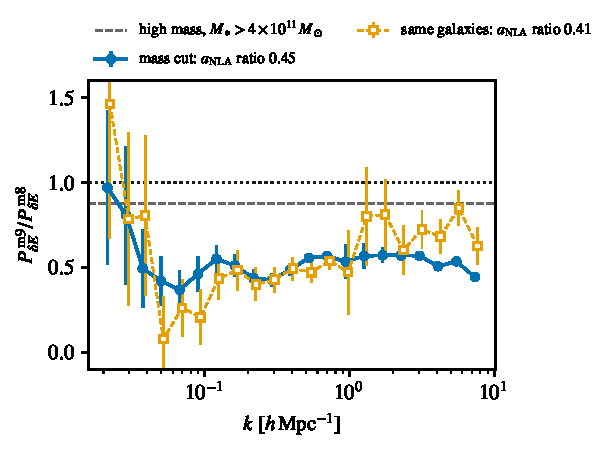
\includegraphics[width=3.5in]{plots/lowmass_ratio/lowmass_ratio.pdf}
  \caption{Ratio of $\PdE$ at m9 (\run{L1\_m9}) to m8 (\run{L1\_m8}) for
    $10.0 < \log\Mstar < 10.41$, $z=0$, unreduced tensor of all bound stars.
    Filled circles: all galaxies in the mass range at each resolution. Open
    squares: the same galaxies paired across the two runs. Dotted: 1; dashed:
    the high-mass ratio of Figure~\ref{fig:m9_m8_ratio}. Errors as in
    Figure~\ref{fig:m9_m8_ratio}.}
  \label{fig:lowmass_ratio}
\end{figure}

\paragraph{The shapes are unrelated, not just noisy.}
The median paired galaxy has \NstarLMnine{} star particles at m9 and
\NstarLMeight{} at m8. The shape correlation between the pairs is \corrLM, and
the median position-angle offset is \paLM, against $45^\circ$ for random
orientations; it stays at \corrLMlow{} to \corrLMhigh{} across m9 star counts
from 10 to above 40, and for centrals matched to $5\,h^{-1}$kpc. The m9 shapes
are also more elongated, $\erms = \ermsLMnine$ against \ermsLMeight.

Counting noise does not explain this. Drawing $N$ points from the same
ellipsoid and measuring the unreduced tensor (Appendix~\ref{app:method}, Method
details) keeps \mcResponseTwenty{} of the alignment at $N = 20$ and adds
\mcNoiseTwenty{} of noise per component, which accounts for the larger $\erms$
but not for a factor 2 loss nor for random orientations. At about 20 particles,
the m9 galaxy is a different object from its m8 counterpart.

\section{What the 2.8 Gpc box adds at low $k$}
\label{sec:lowk}

The fundamental mode $2\pi/L$ of the box is $\kfLtwo\hMpc$ in the 2.8~Gpc box
and $\kfLone\hMpc$ in the 1~Gpc box. Below $k \sim 0.03\hMpc$ the error is set by the number of Fourier
modes, not of galaxies. Figure~\ref{fig:lowk_sn} gives the signal-to-noise of
$\PhE$ per bin. \run{L1\_m8} reaches $\mathrm{S/N} \ge 3$ from
$k = \kSNLone\hMpc$. In the forecast, the 2.8~Gpc box reaches it from
$k = \kSNideal\hMpc$ with galaxies of m8 quality, and from
$k = \kSNmnine\hMpc$ with the galaxies it has, whose signal is half as large
and whose shapes are noisier. The second case also carries the factor 2.2 to
2.5 correction of the previous section.

\begin{figure}[tbp]
  \centering
  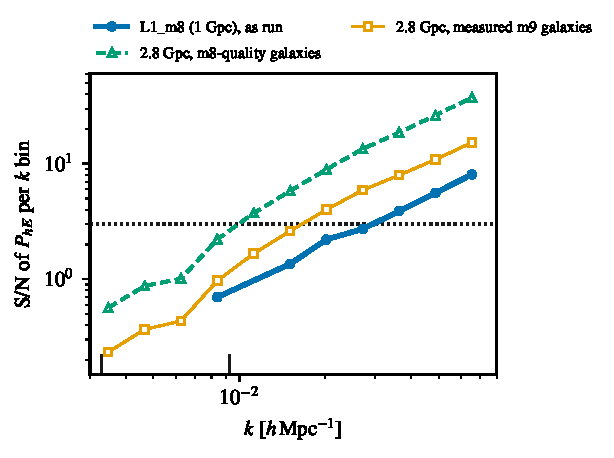
\includegraphics[width=3.5in]{plots/lowk_sn/lowk_sn.pdf}
  \caption{Signal-to-noise of $\PhE$ per $k$ bin at $z = 0$ (Gaussian errors,
    exact mode counts, the 30 logarithmic bins of the pipeline) for
    \run{L1\_m8} as run (thick, circles), the 2.8~Gpc box with the
    \run{L1\_m8} galaxy density, bias, $\anla$ and $\erms$ (dashed,
    triangles), and with the values measured for the m9 sample (thin,
    squares). Dotted: $\mathrm{S/N} = 3$. Ticks at the bottom: the fundamental
    modes of the two boxes.}
  \label{fig:lowk_sn}
\end{figure}

\section{Recommendation}
\label{sec:recommendation}

Keep \run{L1\_m8} for the IA spectra of the paper's sample. At
$k \lesssim 0.03\hMpc$ the alignments are in the linear regime, where the NLA
term of the stitched spectra is reliable. \run{L2p8\_m9} remains useful for
samples with $\log\Mstar > 10.9$ (a 12\% resolution deficit, measurable with
the same-phase pair) and as a check that $\PdE$ follows linear theory down to
$k \simeq 0.008\hMpc$, which its high-mass sample already shows.

\appendix

\section{Method details}
\label{app:method}

\paragraph{Counting-noise Monte Carlo.}
Points are drawn from a Hernquist profile truncated at 20 scale radii,
stretched to axis ratios $(1, q, s)$ with $q \in [0.5, 0.95]$ and
$s \in [0.3, 0.6]$, and rotated at random; 4000 galaxies per $N$. The true
shape is that of the ellipsoid's second moments. The response is
$R = \langle \mathbf{e}_N\cdot\mathbf{e}\rangle / \langle |\mathbf{e}|^2\rangle$, the
factor that multiplies an alignment signal; the extra noise is the rms of
$\mathbf{e}_N - R\,\mathbf{e}$ per component. $R$ is 0.83 at $N=10$, 0.91 at 20,
0.98 at 100.

\paragraph{Low-$k$ forecast.}
For a bin with $N_{\rm m}$ independent modes,
$\sigma^2(\PhE) = [\PhE^2 + (P_{hh} + 1/n)(P_{EE} + \erms^2/2n)]/N_{\rm m}$,
with $\PhE = b\,\anla C_1\rho_{\rm cr}\Omega_m P_{\rm NL}$,
$P_{hh} = b^2P_{\rm NL}$ and $P_{EE} = (\anla C_1\rho_{\rm cr}\Omega_m)^2
P_{\rm NL}$. Mode counts are exact on each box's grid. Galaxy densities scale
with volume from the \run{L1} samples. The high-mass \run{L2p8\_m9} spectrum
measures $\mathrm{S/N} = 5.0$ at $k = 0.011\hMpc$, above the forecast for the
paper's sample because its bias and amplitude are larger.

\section{Numerical checks}
\label{app:checks}

\begin{itemize}
  \item The \run{L1\_m8} low-mass spectrum, rebuilt on the $512^3$ grid from
    the production catalogue, gives $\anla = \anlaLMeight$; the production run
    on $1024^3$ gave $\anlaProd$.
  \item Paired galaxies lie $0.067\Mpch$ apart (median, 99\% below 0.19) with
    a median mass ratio of 0.004~dex; 94\% agree on central or satellite.
  \item The shape correlation is 0.03 for all three tensors in the catalogue
    (unreduced, reduced, within two half-mass radii) and in the $x$ and $y$
    projections.
  \item The particle streaming of \run{L1\_m9} read all \NstarsLnine{} star
    particles; star counts per galaxy agree with SOAP's to within one.
\end{itemize}

\section{Where the code and results are}
\label{app:code}

All under \texttt{flamingo/resolution\_tests/} (its \texttt{README.md} lists the
galaxy catalogues kept outside the repository). The extraction code is
\texttt{flamingo/extraction/}, unchanged.
\begin{center}
  \begin{tabular}{ll}
    \toprule
    result & script $\rightarrow$ output \\
    \midrule
    particle counts & \texttt{particle\_count.py} $\rightarrow$ \texttt{particle\_count.json} \\
    counting noise & \texttt{discreteness\_mc.py} $\rightarrow$ \texttt{discreteness\_mc.json} \\
    high mass & \texttt{restest\_L1m9/run.sh}, \texttt{compare3.py} $\rightarrow$ \texttt{results.json} \\
    high mass, pairs & \texttt{restest\_L1m9/match.py} $\rightarrow$ \texttt{match.json} \\
    low mass & \texttt{lowmass\_L1m9/run.sh}, \texttt{compare.py} $\rightarrow$ \texttt{results.json} \\
    low $k$ & \texttt{lowk\_forecast.py} $\rightarrow$ \texttt{lowk\_forecast.json} \\
    figures & \texttt{notes/flamingo\_m9\_resolution/plots/make\_figure\_data.py} \\
    \bottomrule
  \end{tabular}
\end{center}

\section{Open issues}
\label{app:open}

\begin{itemize}
  \item Only $z = 0$ was tested. At higher redshift the m9 galaxies of the
    sample have fewer particles still, so the deficit is not expected to shrink,
    but it was not measured.
  \item m8 convergence is untested: FLAMINGO has no m7 run. The high-mass
    galaxy-by-galaxy correlation of 0.59 at more than 500 particles indicates
    that m8 shapes at 100 to 250 particles also carry resolution noise.
  \item The errors are mode scatter, underestimated at high $k$ (production
    run caveat); the same-phase ratios have correlated errors that the plotted
    bars ignore.
\end{itemize}

\end{document}
